\documentclass[a4paper]{article}

\usepackage[margin=1in]{geometry} 
\usepackage[hidelinks]{hyperref}
\usepackage{tocloft}
\renewcommand{\cftsecleader}{\cftdotfill{\cftdotsep}}
\renewcommand{\baselinestretch}{1.25} 

\usepackage{minted}
\usepackage{inconsolata}

\usepackage{csquotes}

\usepackage{enumitem}

\usepackage{booktabs}% http://ctan.org/pkg/booktabs
\newcommand{\tabitem}{~~\llap{\textbullet}~~}

\usepackage{graphicx}
\graphicspath{ {./images/} }

\newcommand*{\img}[1]{%
	\raisebox{-.3\baselineskip}{%
		\includegraphics[
		height=\baselineskip,
		width=\baselineskip,
		keepaspectratio,
		]{#1}%
	}%
}

\setcounter{tocdepth}{4}
\setcounter{secnumdepth}{3}

\usepackage{amssymb}
\usepackage{amsmath}
	\DeclareMathOperator*{\argmax}{arg\,max}
	\DeclareMathOperator*{\argmin}{arg\,min}
\usepackage{array}
\usepackage{enumitem}
\usepackage{cellspace}
	\setlength\cellspacetoplimit{4pt}
	\setlength\cellspacebottomlimit{4pt}
\usepackage{framed}

\newcommand\cincludegraphics[2][]{\raisebox{-0.3\height}{\includegraphics[#1]{#2}}}

\usepackage{textcomp}
\newcommand{\textapprox}{\raisebox{0.5ex}{\texttildelow}}

%%% Better lambda 
\usepackage{pifont}
\makeatletter
\newcommand\Pimathsymbol[3][\mathord]{%
	#1{\@Pimathsymbol{#2}{#3}}}
\def\@Pimathsymbol#1#2{\mathchoice
	{\@Pim@thsymbol{#1}{#2}\tf@size}
	{\@Pim@thsymbol{#1}{#2}\tf@size}
	{\@Pim@thsymbol{#1}{#2}\sf@size}
	{\@Pim@thsymbol{#1}{#2}\ssf@size}}
\def\@Pim@thsymbol#1#2#3{%
	\mbox{\fontsize{#3}{#3}\Pisymbol{#1}{#2}}}
\makeatother
% the next two lines are needed to avoid LaTeX substituting upright from another font
\input{utxmia.fd}
\DeclareFontShape{U}{txmia}{m}{n}{<->ssub * txmia/m/it}{}
% you may also want
\DeclareFontShape{U}{txmia}{bx}{n}{<->ssub * txmia/bx/it}{}
% just in case
%\DeclareFontShape{U}{txmia}{l}{n}{<->ssub * txmia/l/it}{}
%\DeclareFontShape{U}{txmia}{b}{n}{<->ssub * txmia/b/it}{}
% plus info from Alan Munn at https://tex.stackexchange.com/questions/290165/how-do-i-get-a-nicer-lambda?noredirect=1#comment702120_290165
\newcommand{\pilambdaup}{\Pimathsymbol[\mathord]{txmia}{21}}

\title{01.112 Machine Learning\\Finals Revision}
\author{Tey Siew Wen}

\date{06 Feb 2020}
\begin{document}
	
\maketitle

\section*{Preface}
Beware notes for these concepts were \textbf{not written}, as I felt that they were pretty self-explanatory when you learn them.

\begin{itemize}
	\item Neural Networks
	\item Generative Models
\end{itemize}

\tableofcontents
\newpage
\section{Background Information}
\subsection{What is Machine Learning}
Machine learning revolves around \textbf{models}, which are trained via certain \textbf{techniques} and \textbf{learning algorithms} that are based on specific \textbf{loss functions}. They produce outputs based on \textbf{predictor functions}.
\subsection{Recap on Convex Functions}
A convex function typically has a U-shape (there are boundary cases where the surface can be flat, though. In that case the function is both convex and concave).\\
\\
\noindent Properties:
\begin{itemize}
	\item $\displaystyle \frac{f(x_1)+f(x_2)}{2} \geq f\left(\frac{x_1+x_2}{2}\right)$
	\item Its local optimum is also a global optimum.
	\item Sum of convex functions is also convex.
\end{itemize}
\noindent Some examples:
\begin{itemize}
	\item $f(x) = (x-1)^2 $
	\item $f(x) = \max(x^2, 2^x)$
	\item $f(x) = |x| - x$
\end{itemize}
\noindent The convexity of empirical risk allows us to find the minimum even in non-realizable case.
\subsection{Empirical Risk}
Defined as the average loss on the training examples.
\begin{align*}
	R_n(\theta) = \frac{1}{n} \sum_{t=1}^{n} \text{Loss}_h(y^{(t)}\theta\cdot x^{(t)})
\end{align*}
\subsection{Loss Functions}
\begin{table}[H]
	\centering
	\begin{tabular}{|l|c|}
		\hline
		\multicolumn{1}{|c|}{\textbf{Loss function}} & \textbf{$\text{Loss}_h(z)$} \\ \hline
		Squared Euclidean/ Least Squares             & $\frac{1}{2}z^2$            \\ \hline
		Zero-one loss                                &                             \\ \hline
		Hinge Loss                                   & $\max{(1-z , 0)}$           \\ \hline
	\end{tabular}
\end{table}
\begin{figure}[H]
	\centering
	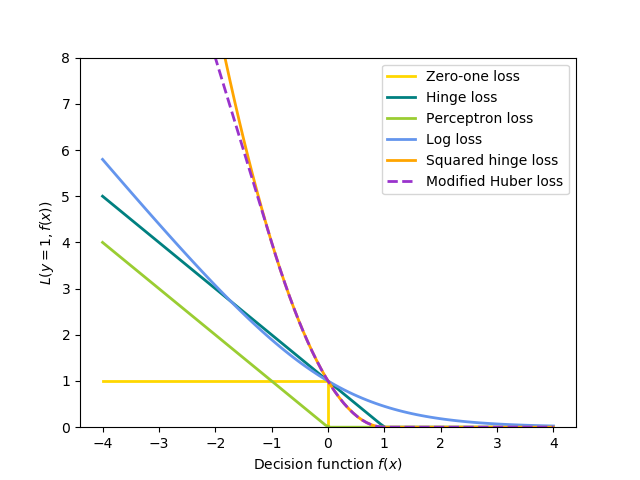
\includegraphics[width=0.7\linewidth]{sgd_loss_functions}
	\label{fig:sgdlossfunctions}
\end{figure}
\subsection{Types of Machine Learning}
\begin{framed}
	\begin{displayquote}
		Notice the resemblance in the problems from each category of tasks.
	\end{displayquote}
\end{framed}
\textbf{Supervised Tasks}
\begin{itemize}
	\item Classification $f: R^n \rightarrow { 1,\ldots, k }$
	\begin{itemize}[label=$\circ$]
		\item LR, SVM, Perceptron NB
	\end{itemize}
	\item Regression: $f: R^n \rightarrow R^m$
	\begin{itemize}[label=$\circ$]
		\item Ridge Regression, Logistic Regression
	\end{itemize}
	\item Structured Prediction: $f: S_1 \rightarrow S_2$ where $\text{size}(S_1) >\text{size}(S_2)$
	\begin{itemize}[label=$\circ$]
		\item HMM, CRF, Structured Perceptron, Structural SVM
	\end{itemize}
\end{itemize}
\textbf{Unsupervised Tasks}
\begin{itemize}
	\item Clustering: $f: R^n \rightarrow { 1,\ldots,k }$
	\begin{itemize}[label=$\circ$]
		\item K-means, EM
	\end{itemize}
	\item Dimensionality Reduction: $f: R^n \rightarrow R^m$
	\begin{itemize}[label=$\circ$]
		\item PCA, LDA, Autoencoder
	\end{itemize}
	\item Structured Prediction: $f: S_1 \rightarrow S_2$
	\begin{itemize}[label=$\circ$]
		\item Unsupervised HMM
	\end{itemize}
\end{itemize}
\newpage
\section{Introduction to Machine Learning}
\boxed{\texttt{algorithms}} \boxed{\texttt{tasks}} \boxed{\texttt{performance}} \boxed{\texttt{experience}}\\
\\
\noindent Definition of Machine Learning: ML is programming computers to optimize a \textbf{performance criterion} using example data or past experience.\\
\\
ML has been studied since computers came out, but back then the amount of existing data is insufficient to do any useful ML, so it died quickly by 1970s. It is only now in the Big Data, IOT age that data is ever so abundant,and with enhanced computational power, ML can be applied meaningfully to these data to solve real-world problems that were previously too complex to be analyzed/ computationally difficult. Using ML, we aim to build models that are useful \textbf{approximations} of the relationship between input data and output data. After all, we can never tell if there is ever an absolute relationship between any sets of data.\\
\\
\noindent We usually denote each feature (column) vector of dimension $d$ as such:
$$ x = x[x_1,\ldots,x_d]^T \subset R^d $$
$$\begin{aligned}
x^{(1)}, x^{(2)},\ldots, x^{(n)}:& \textsf{ training examples} \\ y^{(1)},y^{(2)},\ldots,y^{(n)}:&\textsf{ the corresponding labels} \end{aligned} $$
\noindent If x is used to denote the original object (e.g. image), then we would use the following notation to denote the feature vector:
$$ \phi(x) \subset R^d $$
\subsection{Key Aspects of Learning Problems}
\begin{enumerate}
	\item Data: could be Biased
	\item Modelling: Set of Classifiers $H(x)$
	\item Optimizing: Learning Algorithm / Performance Criterion
	\begin{itemize}[label=$\circ$]
		\item Each algorithm comes with its assumptions
	\end{itemize}
\end{enumerate}
\newpage
\section{Types of Machine Learning}
\subsection{Based on Learner's role}
\begin{itemize}
	\item Passive Learning
	\begin{itemize}[label=$\circ$]
		\item Traditionally, learning algorithms have been passive learners in which they just take the data to produce hypothesis/model.
	\end{itemize}
	\item Active Learning
	\begin{itemize}[label=$\circ$]
		\item Active Learners can query the environment by asking questions/ performing experiments.
		\item But it is difficult to account for the cost of queries/ query the environment optimally.
	\end{itemize}
\end{itemize}
\subsection{Based on Information/Dataset Available}
\begin{enumerate}
	\item \textbf{\textit{Supervised Learning:}} using labelled data
	\begin{itemize}[label=$\circ$]
		\item Classification (discrete values)
		\item Regression (real values)
	\end{itemize}
	\item \textbf{\textit{Unsupervised Learning:}} using unlabelled data
	\begin{itemize}[label=$\circ$]
		\item Clustering
		\item Probability Distribution Estimation
		\item Finding Association In Features
		\item Dimension Reduction
	\end{itemize}
	\item \textbf{\textit{Semi-supervised Learning:}} using a small subset of labelled data with a large amount of unlabelled data for learning
	\item \textbf{\textit{Reinforcement Learning:}} Using state spaces
	\begin{itemize}[label=$\circ$]
		\item Decision Making (robotics, games like DOTA)
	\end{itemize}
	\item \textbf{\textit{Transfer Learning:}} Reusing trained filters for other models
\end{enumerate}
\subsubsection{Supervised Learning}
\paragraph{Classification}\mbox{}\\
Steps to solving a supervised learning problem
\begin{enumerate}
	\item Decide what the input-output pairs
	\item Decide how to encode inputs and outputs
	\item Choose a class of hypothesis (modelling)
	\item Choose error function to define best hypothesis
	\item Choose algorithm for searching efficiently through the space of hypotheses (optimizing)
\end{enumerate}
\subsubsection{Unsupervised Learning}
\paragraph{Clustering}\mbox{}\\
Need to know approximately how many clusters of data is expected.
\paragraph{Dimensionality Reduction: Sub-space Learning}\mbox{}\\
\\
\underline{The importance of Dimensions}\\
\\
Say Boy A is training for IPPT and he records all the timings he takes to train 2.4km. It will result in 1D plot on the number line. But if he adds in the readings by his friend and have his records be differentiated, the result will be a 2D plot. If he adds a 3rd friend, the graph will become a 3D plot. The 4th friend onwards will be a Nth-D plot but it cannot be visualized anymore.\\
\\
\noindent For a fitness trainer that sees data like this, sometimes he doesn't really care who ran how long but he just wants to see the duration of each practice run that has taken place and how the data varies. So for such a problem, we can perform \textbf{Principal Component Analysis} to reduce the dimensions involved and still get useful information out it.\\
\\
\noindent \underline{Principal Component Analysis}\mbox{}\\
Definition of PCA: A statistical procedure that uses an orthogonal transformation to convert a set of observations of possibly correlated variables (entities each of which takes on various numerical values) into a set of values of \textbf{linearly uncorrelated} variables called \textit{principal components}.
\begin{framed}
	\begin{displayquote}
		PCA works optimally only in the situation where the correlations are linear, which is most of the time an approximation. Otherwise do something to transform the data to linear variables or perform Nonlinear dimensionality reduction.
	\end{displayquote}
\end{framed}
\begin{itemize}
	\item As described in the IPPT example, PCA can be used to convert the Original Data Space to Component Space.
	\item These principal components mark the axes for the new plot with reduced dimensions. The first principal component (PC1) is the axis that spans the most variation in data, followed by PC2 with the 2nd most variation and so on.
\end{itemize}
Orthogonal transformation is performed via \href{https://en.wikipedia.org/wiki/Eigendecomposition_of_a_matrix}{Eigenvalue decomposition} of a data covariance/ correlation matrix (must be diagonalizable):\\
\mbox{}\\
\noindent Let A be a square n × n matrix with n linearly independent eigenvectors $q_i$ (where i = 1, $\ldots$ , n).\\
Then A can be factorized as
$$Av =\pilambdaup v$$
$$Q = Q$$
$$A = Q\pilambdaup Q^{-1} $$ $$ \text{Q: square n × n matrix whose ith column is the eigenvector of A}$$ $$ \text{A: the diagonal matrix whose diagonal elements are the corresponding eigenvalues } A_{ii} = \pilambdaup_i. $$
\subsubsection{Reinforcement Learning}
\begin{itemize}
	\item \textit{Curse of Dimensionality:} all data points appear to be sparse and dissimilar in many ways, which prevents common data organization strategies from being efficient. This results in more complicated control problems to not fit enumerable states even if we discretize them.
	\item \textit{Assumes Markov Property:} The future does not depend on the past. The conditional probability distribution of future states of the process (conditional on both past and present values) depends only upon the present state.
	\begin{itemize}[label=$\circ$]
		\item If there are consistent unknown factors that influence result, and could logically be deduced - maybe from history of state or actions - but are excluded from the state representation, the agent may fail to learn.
	\end{itemize}
\end{itemize}
\section{Why Study ML}
\subsection{Engineering reasons for studying ML}
\begin{itemize}
	\item Improving existing programs via:
	\begin{itemize}[label=$\circ$]
		\item Instruction scheduling and register allocation in compilers
		\item Combinatorial Optimization Problems
	\end{itemize}
	\item Solving tasks that require adaptive systems
	\begin{itemize}[label=$\circ$]
		\item where humans can perform the task but cannot explain how e.g. speech/handwriting recognitiion, intelligent UIs
		\item desired function changes frequently e.g. predict stock prices
		\item each user needs a customized function e.g. news filtering
	\end{itemize}
	\item We don't want to hand code a lot of programs
	\item Performing tasks where there is no human expert
\end{itemize}
\subsection{Scientific reasons for studying ML}
\begin{itemize}
	\item Discover knowledge \& patterns in highly dimensional, complex data
	\item Understanding the process of learning
\end{itemize}
\newpage
\section{Linear Classification}
A classifier $h$ partitions space into decision regions that are separated by decision boundaries. In each region, all the points map to the same label. For linear classifiers, these regions are half spaces.\\
\\
A linear classifier $h$ takes the following form
$$ h(x;\theta) = \text{sign}(\theta^Tx) = \text{to add}$$
\subsection{Algorithms}
\subsubsection{Perceptron Update Rule (Mistake-Driven Updates)}
\paragraph{Theorem}\mbox{}\\
The perceptron update rule converges after a finite number of mistakes when the training examples are linearly separable through origin. This implies that zero training error can be achieved using perceptron update rule for linearly separable training examples.
\begin{framed}
	\begin{displayquote}
		The algorithm will not converge for non-linearly separable data! Refer to Stochastic (Sub)-Gradient Descent instead for such data.
	\end{displayquote}
\end{framed}
\paragraph{How it works}\mbox{}\\
Initialize weight $\theta = 0$. For each training sample $t$ in $S_n$, classify the instance with mistake driven updates. The Perceptron Update Rule will terminate when:
\begin{itemize}
	\item Training error is 0 (Realizable)
	\item Predetermined number of iterations is completed (Non-realizable)
\end{itemize}
A mistaken is recognized with the following condition and the weight is updated as such: $$\begin{aligned} \text{Mistake Condition: } &y^t(\theta\cdot x^t) \leq 0 \quad \text{Update Rule:} &\theta^{(k+1)} = \theta^{(k+1)} = y^{(t)}x^{(t)} \end{aligned}$$
$y^t(\theta\cdot x^t)$ then becomes more positive and eventually becomes $> 0$ (Realizable). If the prediction is correct, continue.
\paragraph{Offset}\mbox{}\\
\begin{itemize}
	\item Set default prediction to +1/-1.
	\item The hyper-plane $\theta\cdot x + \theta_0$ is parallel to \item $\theta\cdot x = 0$.
	$\theta$ is still orthogonal to the decision boundary
	\item For training examples that are linearly separable through origin, they would also be linearly separable with offset. However, the converse is not true.
\end{itemize}
\begin{figure}[H]
	\centering
	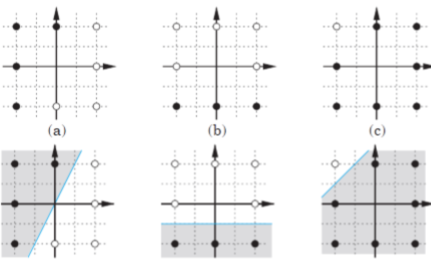
\includegraphics[width=0.5\linewidth]{images/not_linear_separable_through_origin}
	\label{fig:notlinearseparablethroughorigin}
\end{figure}
\subsubsection{Gradient Descent}
Instead of checking if the value is classified wrongly, gradient descent aims to minimize the loss $R_n(\theta)$. 

$$ \nabla_\theta R_n(\theta) =\frac{1}{n} \sum_{t=1}^n \max\{1 - y^{(t)} (\theta\cdot x^{(t)}), 0 \}  $$

\noindent We minimize the loss by finding $\nabla_\theta R_n(\theta)$. 

\begin{align*}
\nabla_\theta R_n(\theta) =& \nabla_\theta \text{Loss}_h(y^{(t)}\theta\cdot x^{(t)}) \\
=& \nabla_\theta(1-y^{(t)}\theta\cdot x^{(t)}) \\
=& -y^{(t)}x^{(t)}
\end{align*}
For values that are classified wrongly, the gradient will point in the direction where the error $R_n(\theta)$ increases, so we update the weight in the opposite direction and descend from the point accordingly. We will also add a learning rate $\alpha$ to control the rate of descent.\\
\\
\noindent Thus the weight will be updated as such $$ \begin{aligned} \theta^{(k+1)} = & \theta^{(k)} - \alpha_k\nabla_\theta R_n(\theta)_{\theta=\theta^{(k)}} \ \theta^{(k+1)} = & \theta^{(k)} + \alpha_k y^{(t)}x^{(t)} \end{aligned} $$
\paragraph{Limitations}
\begin{itemize}
	\item However, $R_n(\theta)$ is not differentiable everywhere as hinge loss functions are piece-wise linear.
	\item There are several possible gradients at the kinks, which are collectively defined as sub-differential.
	\item To minimize $R_n(\theta)$, we randomly select one possible gradient.
\end{itemize}
\begin{figure}[H]
	\centering
	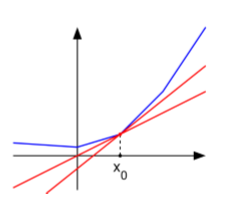
\includegraphics[width=0.3\linewidth]{images/kink}
	\label{fig:kink}
\end{figure}
If there are many training examples, it is better to use Stochastic Gradient Descent (SGD).
\subsubsection{Stochastic (Sub)-Gradient Descent}
\begin{itemize}
	\item Random sample avoid oscillations
	\item Keep track of best solution (the weights where the loss is minimum).
	\item Near mistakes are penalized
	\item Decreasing learning rate, for smaller updates, $\alpha_k = 1/(k+1)$
\end{itemize}
\paragraph{How it works}
\begin{enumerate}
	\item Initialize weight $\theta$ = 0
	\item Select random data point, t.
	\item If $y^{(t)}\theta^{(k)} \cdot x^{(t)} \leq 1$ then update weight.
	\item Repeat steps 2-3 until stopping criterion is met.
\end{enumerate}
\subsubsection{Closed Form Solution}
Using least squares criterion, we can also minimize empirical risk directly by setting gradient to zero.

$$ \begin{aligned} \nabla_\theta R_n(\theta) &= -b + A\theta \end{aligned} $$ $$ \begin{aligned} \text{where } &b = \frac{1}{n}\sum_{t=1}^n y^{(t)}x^{(t)} = \frac{1}{n}X^TY, \ & A = \frac{1}{n}\sum_{t=1}^n x^{(t)}\cdot (x^{(t)})^T = \frac{1}{n}X^TX \end{aligned} $$
\textbf{If A is invertible}, we can find the weight directly:
$$ \begin{aligned}
\theta &= A^{-1}b \ &= \left(\frac{1}{n}X^TX\right)^{-1}\left(\frac{1}{n}X^T\vec{y}\right) \end{aligned} $$
\begin{itemize}
	\item Note the cost of inverting matrix $A$ is usually $O(d^3)$ for normal gradient descent.
\end{itemize}
\textbf{If A is not invertible}, the training data will not be able to guide the model on setting parameter directions. Hence, we can choose to modify the estimation criterion, the mean squared error in this case, by adding a regularizatioon term. The regularization term $\pilambdaup$ shifts emphasis away from the training data.
\begin{itemize}
	\item Larger values of $\pilambdaup$ will result in larger training error, but lower generalization error $J_n(\theta)$ as we are less swayed by noisy data. So, it is harder to over-fit to training data.
	\item But as $\pilambdaup$ increases too much, it will bias the parameters too strongly towards zero.
\end{itemize}
Let's choose $\displaystyle \frac{||\theta||^2}{2}$ as the penalty for easier solvability. This means that we will aim to minimize
$$ J_{n,\pilambdaup} = \frac{\pilambdaup}{2}||\theta||^2 + R_n(\theta)$$ This is known as Ridge Regression.
\subsubsection{Ridge Regression}
\paragraph{Using Gradient Descent}\mbox{}\\
Using GD/SGD for learning parameters in this technique, the weight will be updated as such

$$ \theta^{k+1} = (1-\pilambdaup\alpha_k)\theta^{k} + \alpha_k(y^{(t)} - \theta\cdot x^{(t)})x^{(t)} $$

\noindent The new factor $(1-\pilambdaup\alpha_k)$ helps to shrink the parameters $\theta^{(k)}$ towards zero during each update.
Without regularization i.e. $\pilambdaup = 0$, it will look the same as the original gradient descent.
\begin{figure}[H]
	\centering
	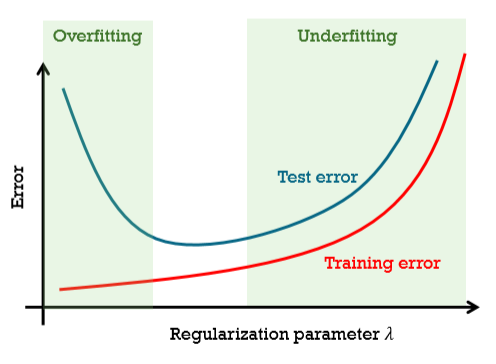
\includegraphics[width=0.4\linewidth]{images/effects_of_regularization}
	\label{fig:regularization}
\end{figure}
\paragraph{Closed Form Solution}\mbox{}\\
The regularization term only modifies the matrix $A = \lambda I + \left(\displaystyle \frac{1}{n}\right)X^TX$, where $I$ is the identity matrix. $$ \theta = (n\pilambdaup I + X^TX)^{-1} X^TY $$ The identity matrix is always invertible if $\pilambdaup >$ 0.
\newpage
\section{Clustering}
\begin{itemize}
	\item Unsupervised learning
	\item Cluster: collection of similar data points, and is sufficiently different from other groups.
	\item Criterion for selecting clusters \& representatives
	\begin{itemize}[label=$\circ$]
		\item Cosine Similarity: $\displaystyle \frac{x^{(i)}\cdot x^{(j)}}{||x^{(i)}||\cdot ||x^{(j)}||}$
		\item Euclidean Distance: $||x^{(i)}|| - ||x^{(j)}||$
	\end{itemize}
\end{itemize}
\subsection{K-means}
\subsubsection{Cost of Clustering}
$$ \text{cost}(C_1\ldots C_k, z^{(1)}\ldots z^{(k)}) = \sum_{j=1\ldots k}\sum_{i\Subset C_j} ||x^{(i)} - z^{(j)} ||^2 $$

$$ \text{cost}(z^{(1)}\ldots z^{(k)}) = \sum_{i=1\ldots n} \min_{j=1\ldots k} ||x^{(i)} - z^{(j)} ||^2 $$
\subsubsection{How it works}
\begin{enumerate}
	\item Choose the number of clusters $k$
	\item Place the centroids $c_1, c_2, \ldots c_k$ randomly
	\item For each data point $x_i$:
	\begin{itemize}[label=$\circ$]
		\item Find the nearest centroid $(c_1, c_2 \ldots c_k)$
		\item Assign the point to that cluster
	\end{itemize}
	\item For each cluster j = $1..k$
	\begin{itemize}[label=$\circ$]
		\item New centroid = mean of all points assigned to that cluster $$z^{(j)} = \frac{1}{|C_j|} \sum_{i \Subset C_j} x^{(i)}$$
	\end{itemize}
	\item Repeat steps 4 and 5 until
	\begin{itemize}[label=$\circ$]
		\item convergence (when we find a clustering that minimizes the cost of clustering)
		\item or until the end of a fixed number of iterations.
	\end{itemize}
\end{enumerate}
Each iteration requires $O(kn)$ operations, and necessarily lowers the cost of clustering, the sum of costs of individual clusters.
\subsection{K-medoids}
\subsubsection{Choosing k}
We should choose the value of k that results in the highest relative drop in the cost (which corresponds to an “elbow” in the graph capturing as a function of $k$).
\subsubsection{How it works}
\begin{enumerate}
	\item Choose the number of clusters $k$
	\item Choose the exemplars $z_1, z_2, \ldots, z_k$ randomly out of the data points (or given otherwise)
	\item For each data point $x_i$, other than the centroids:
	\begin{itemize}[label=$\circ$]
		\item Calculate the distance to each exemplar $z_1, z_2, \ldots, z_k$
		\item Add the data point to the cluster that contains $z^{(j)}$ which is nearest to the point $x_i$.
	\end{itemize}
	\item Set new exemplar $z^{(j)}$ to be the point in $C^j$ that minimizes $\sum_{i\Subset C^j} d(x^{(i)},z^{(j)})$
	\item Repeat steps 3-4 until no further change in cost.
\end{enumerate}
\subsection{Difference between K-means and K-medoids}
\begin{table}[H]
	\centering
	\begin{tabular}{|l|l|}
		\hline
		\multicolumn{1}{|c|}{\textbf{K-medoids}}                                                                                                                         & \multicolumn{1}{c|}{\textbf{K-means}}                                                                                                                                                  \\ \hline
		\begin{tabular}[c]{@{}l@{}}Applicable to arbitrary objects and distance functions \\ (e.g. categorical data)\end{tabular}                                        & \begin{tabular}[c]{@{}l@{}}Not applicable for arbitrary objects  \\ and distance functions\end{tabular}                                                                                                                             \\ \hline
		\begin{tabular}[c]{@{}l@{}}Less sensitive to noisy data \\ $\Rightarrow$ Mediod is less influenced by outlier than a mean.\end{tabular}       & More sensitive to noisy data                                                                                                                                                           \\ \hline
		\begin{tabular}[c]{@{}l@{}}Applicable when true data points are unavailable \\ and only their pair-wise distances are provided\end{tabular}           & Not applicable if true data points are not available                                                                                                                                \\ \hline
		Applicable to both continuous and discrete domains                                                                                                           & \begin{tabular}[c]{@{}l@{}}Only applicable to the continuous domain since\\the mean is not necessarily a data point.\end{tabular} \\ \hline
		\begin{tabular}[c]{@{}l@{}}Longer run time, especially for large and random\\ datasets. Harder than computing the average.\end{tabular} & Shorter run time                                                                                                                                                                       \\ \hline
		\begin{tabular}[c]{@{}l@{}}Has no statistical meaning;\\ Neither a median nor geometric median\end{tabular}                                                      & Has a true geometrical and statistical meaning                                                                                                                                         \\ \hline
	\end{tabular}
\end{table}
\subsubsection{Similarities between K-means and K-medoids}
\begin{itemize}
	\item Each iteration decreases the cost
	\item The algorithm always converges
	\item Different starts gives different final answers
	\item It does not achieve the global minimum
\end{itemize}
\newpage
\section{Support Vector Machines (SVMs)}
\subsection{Adding Slack Variables}
Sometimes we get data which has two classes that are mostly separated except some small training data where the two categories overlap. In such cases, we would like to allow some points to intentionally be misclassified so as classify the rest correctly.\\
\\
To do so, for each training data point we can define a variable that measures the distance of the point to its marginal hyperplane, $\xi_t$, in terms of the hinge loss function.

\begin{align*}
	\xi_t &= \text{Loss}_h(y^{(t)}(\theta\cdot x^{(t)} + \theta_0))\\
	 &= \max \{1-y^{(t)}(\theta\cdot x^{(t)}),0 \}
\end{align*}
\begin{figure}[H]
	\centering
	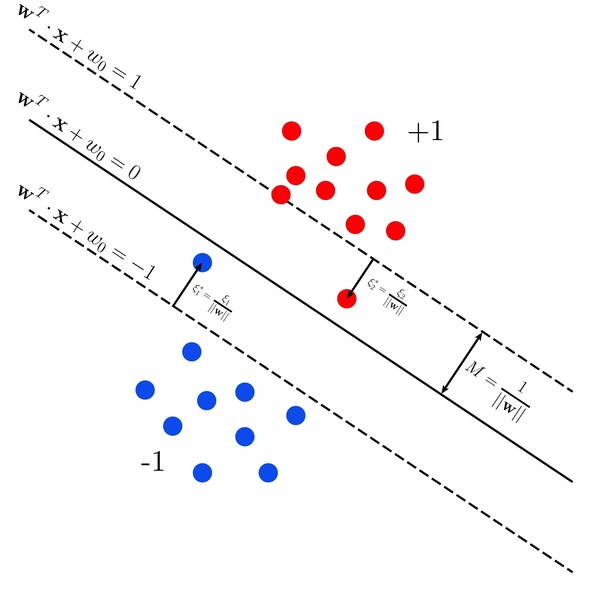
\includegraphics[width=0.5\linewidth]{images/slack_variable}
	\label{fig:slack_variable}
\end{figure}
\noindent We can define a separating hyperplane by minimizing such errors $\xi_i$:

$$ \min_{\theta,\theta_0,\xi} { \sum_{i=1}^N \xi_i } $$

\noindent Each individual training point has a different but parallel marginal hyperplane.

\begin{align*}
	 \theta\cdot x + \theta_0 \geq 1 - \xi_i &\quad \text{if } y_i = +1\\
	 \theta\cdot x + \theta_0 \leq -1 + \xi_i &\quad \text{if } y_i = -1
\end{align*}
Combining these 2 equations we yield a single equation for the constraint of primal problem. $$ y^{(i)}(\theta\cdot x^{(i)} + \theta_0) \geq 1 -\xi_i $$
\newpage
\subsubsection{Updated Primal Problem}
$$ \min \frac{\lambda}{2}||\theta||^2 + \sum_{t=1}^n \xi_t$$
\begin{align*}
	\text{such that } y^{(i)}(\theta\cdot x^{(i)} + \theta_0) \geq 1 -\xi_i,\ \xi\geq 0,\ t=1\ldots n
\end{align*}
Here, the slack variables are simply encoding the \textbf{hinge loss in the primal formulation}.
\subsubsection{Updated Dual Formulation}
The Dual Problem remains the same, except that we limit how large the Langrange multipliers $\alpha_t$ can become.
\begin{itemize}
	\item Also the larger the value of $\lambda$ (the more we want to expand the margin at the expense of the constraints), the smaller the resulting $\alpha_t$ must be.
\end{itemize}
$$ \max \sum_{i=1}^n \alpha_t - \frac{1}{2} \sum_{i=1}^n\sum_{j=1}^n \alpha_i \alpha_j y^{(i)}y^{(j)}(x^{(i)}) $$
$$ \text{subject to } 0 \leq \alpha_t \leq \frac{1}{\pilambdaup},\ \sum_{i=1}^n \alpha_i y^{(i)} = 0 $$
\subsubsection{Complementary slackness constraints}
\begin{align*}
	&\hat{\alpha}_i = 0 \rightarrow &\text{non-support vectors: } \ y^{(i)} (\sum{j=1}^n \hat{\alpha}_j y^{(j)}(x^{(j)} \cdot x^{(i)}) + \hat{\theta}_0) \geq 1\\
	&\hat{\alpha}_i \Subset \left(0,\frac{1}{\pilambdaup}\right) \rightarrow &\text{support vectors: }\ y^{(i)} (\sum{j=1}^n \hat{\alpha}_j y^{(j)}(x^{(j)} \cdot x^{(i)}) + \hat{\theta}_0) = 1 \\
	&\hat{\alpha}_i = \frac{1}{\pilambdaup} \rightarrow &\text{margin violations: }\ y^{(i)} (\sum{j=1}^n \hat{\alpha}_j y^{(j)}(x^{(j)} \cdot x^{(i)}) + \hat{\theta}_0) \leq 1  
\end{align*}
\noindent We can use $\alpha_i$ that lies in the interior of possible values to reconstruct $\hat{\theta}_0$.
\newpage
\section{Mixture Models and Expectation Minimization}
\subsection{Spherical Gaussian}
Spherical Gaussian Distribution is a simple spherically symmetric distribution around the centroid/mean $\mu$. Given:

\begin{itemize}
	\item $x$: Point
	\item $\mu$: Mean
	\item $\sigma$: Variance
	\item $d$: Dimension
\end{itemize}
The distribution can be represented by a circle centered at mean $\mu$ with radius $\sigma$. We can generate points from the following spherical Gaussian Distribution, each with a likelihood of

\begin{align*}
	 P (x|\mu, \sigma^2) &= N(x;\mu,\sigma^2I)\\
	 &= \frac{1}{(2\pi\sigma^2)^{d/2}}\text{exp}\left(-\frac{1}{2\sigma^2}||x-\mu||^2\right)
\end{align*}

\subsubsection{Overall Objective Function}

We try to find the best Gaussian that fits the data with the criterion of maximum likelihood (ML). The likelihood of the training data is calculated as follows:

\begin{align*}
	\ell(S_n|\mu, \sigma^2) &= \prod_{t=1}^n p(x^{(t)}|\mu,\sigma^2)\\
	&= \sum_{t=1}^n \log p(x^{(t)} | \mu,\sigma^2)\\
	&= \sum_{t=1}^n [-\frac{d}{2}\log(2\pi\sigma^2) - \frac{1}{2\sigma^2}||x^{(t)} - \mu||^2]\\
	&= -\frac{dn}{2}\log(2\pi\sigma^2) - \frac{1}{2\sigma^2} \sum_{t=1}^n ||x^{(t)} - \mu||^2
\end{align*}

\noindent To minimize this function and the corresponding Maximum Likelihood Estimators, we find the gradients respective to the parameters $\mu, \sigma^2$ and equate them to 0.

$$ \frac{\partial\ell(S_n|\mu,\sigma^2)}{\partial\mu} = 0 $$ 
$$ \frac{\partial\ell(S_n|\mu,\sigma^2)}{\partial\sigma^2} = 0 $$

\noindent Deriving maximum likelihood estimator of $\mu$, $\hat{\mu}$:
\begin{align*}
	\frac{\partial\ell(S_n|\mu,\sigma^2)}{\partial\mu} &= -\frac{1}{2\sigma^2} \cdot 2 \cdot \sum_{t=1}^n \vec{\mu} - \vec{x}^{(t)}\\
	&= \vec{0} 
\end{align*}
$$ \vec{\mu} = \frac{1}{n}\sum_{t=1}^n \vec{x}^{(t)} $$
\newpage
\noindent Deriving maximum likelihood estimator of $\sigma^2$, $\hat{\sigma^2}$:

\begin{align*}
	\frac{\partial\ell(S_n|\mu,\sigma^2)}{\partial\sigma^2} &= -\frac{dn}{2}\cdot\frac{1}{\sigma^2}\cdot 2\pi - \frac{1}{2\sigma^4}\sum_{t=1}^n||x^{(t)} - \mu||^2\\
	\frac{dn}{2}\cdot\frac{1}{\sigma^2} &= \frac{1}{2\sigma^4}\sum_{t=1}^n||x^{(t)} - \mu||^2\\
	dn &= \frac{1}{\sigma^2}\sum_{t=1}^n||x^{(t)} - \mu||^2\\
	\hat{\sigma^2} &= \frac{1}{dn} \sum_{t=1}^n||x^{(t)} - \mu||^2
\end{align*}

\subsection{Mixture of Gaussians}
When the data are best described by multiply clusters instead of one, we need to specify multiple Gaussians, each for one cluster. Assuming $k$ clusters is optimal for describing the data,

$$ P(x| \mu^{(i)}, \sigma_i^2), \text{for } i = 1,\ldots,k $$

\noindent But we don't have the respective $\mu^{(i)}, \sigma_i^2$, so we have to somehow evaluate the probability each data point $x$ could come as sample from our mixture model, and adjust the model parameters so as to increase this probability. Each $x$ could be generated from any cluster, just with different probabilities.

\noindent For easier representation, we let $\theta$ specify all parameters for the mixture model:

$$ \theta = \{\mu^{(1)},\ldots, \mu^{(k)}, \sigma^2_1,\ldots,\sigma^2_k, p_1,\ldots, p_k \} $$

\noindent where $p_1, \ldots, p_k$ specify the frequency of points we would expect to see in each cluster.

\subsubsection{Labelled Case}

If data points are already labelled (assigned to a single cluster), we could estimate the Gaussian models same as before, and even evaluate the cluster sizes based on the actual number of points.\\
\\
\noindent Let $\delta(i|t)$ be an indicator that tells us whether $x^{(t)}$ should be assigned to cluster $i$.

\begin{itemize}
	\item $\delta(i|t) = 1$, if $x^{(t)}$ is assigned to $i$
	\item $\delta(i|t) = 0$, otherwise
\end{itemize}

\paragraph{Maximum Likelihood Objective}
$$\sum_{t=1}^n\left[\sum_{i=1}^k \delta(i|t)\log\left(p_i\cdot p(x^{(t)}|\mu^{i}, \sigma^2_i)\right)\right]$$

\noindent Here, the inner summation selects the Gaussian that we should use to generate the corresponding data point consistent with the assignments.\\
\\
\noindent We can exchange the summations to demonstrate that the Gaussians can be solved separately from each other. The terms inside the bracket now represents the objective for all points in $i$-th cluster.

$$ \sum_{i=1}^k\left[\sum_{t=1}^n \delta(i|t)\log(p_i\cdot p(x^{(t)}|\mu^{i}, \sigma^2_i))\right] $$

\noindent Updating Model Parameters: 
\begin{align*}
	\text{Number of points assigned to cluster i: } &\hat{n}_i = \sum{t=1}^n \delta(i|t)\\
	\text{Fraction of points in cluster i: } &\hat{p}_i = \frac{\hat{n_i}}{n}\\
	\text{Mean of points in cluster i: } &\hat{\mu}^{(t)}_i = \frac{1}{n}\sum_{t=1}^n \delta(i|t)x^{(t)}\\
	\text{Mean squared spread in cluster i: } &\hat{\sigma^2}_i = \frac{1}{d\hat{n_i}}\sum{t=1}^n \delta(i|t)||x^{(t)}-\hat{\mu}^{(i)}||^2
\end{align*}

\subsubsection{Unlabelled Case}
Now $\delta(i|t)$ is not given, but we can apply the EM-algorithm to derive the respective $\delta(i|t)$.

\subsection{Estimating Mixtures: the EM-Algorithm}
We can use an iterative algorithm known as Expectation Maximization algorithm.\\
\\
\noindent Here are some relevant slides from \href{https://www.youtube.com/watch?v=REypj2sy_5U&list=PLBv09BD7ez_4e9LtmK626Evn1ion6ynrt}{\textcolor{blue}{a good video series by Victor Lavrenko}} on EM that I recommend you to watch.

\begin{figure}[H]
	\centering
	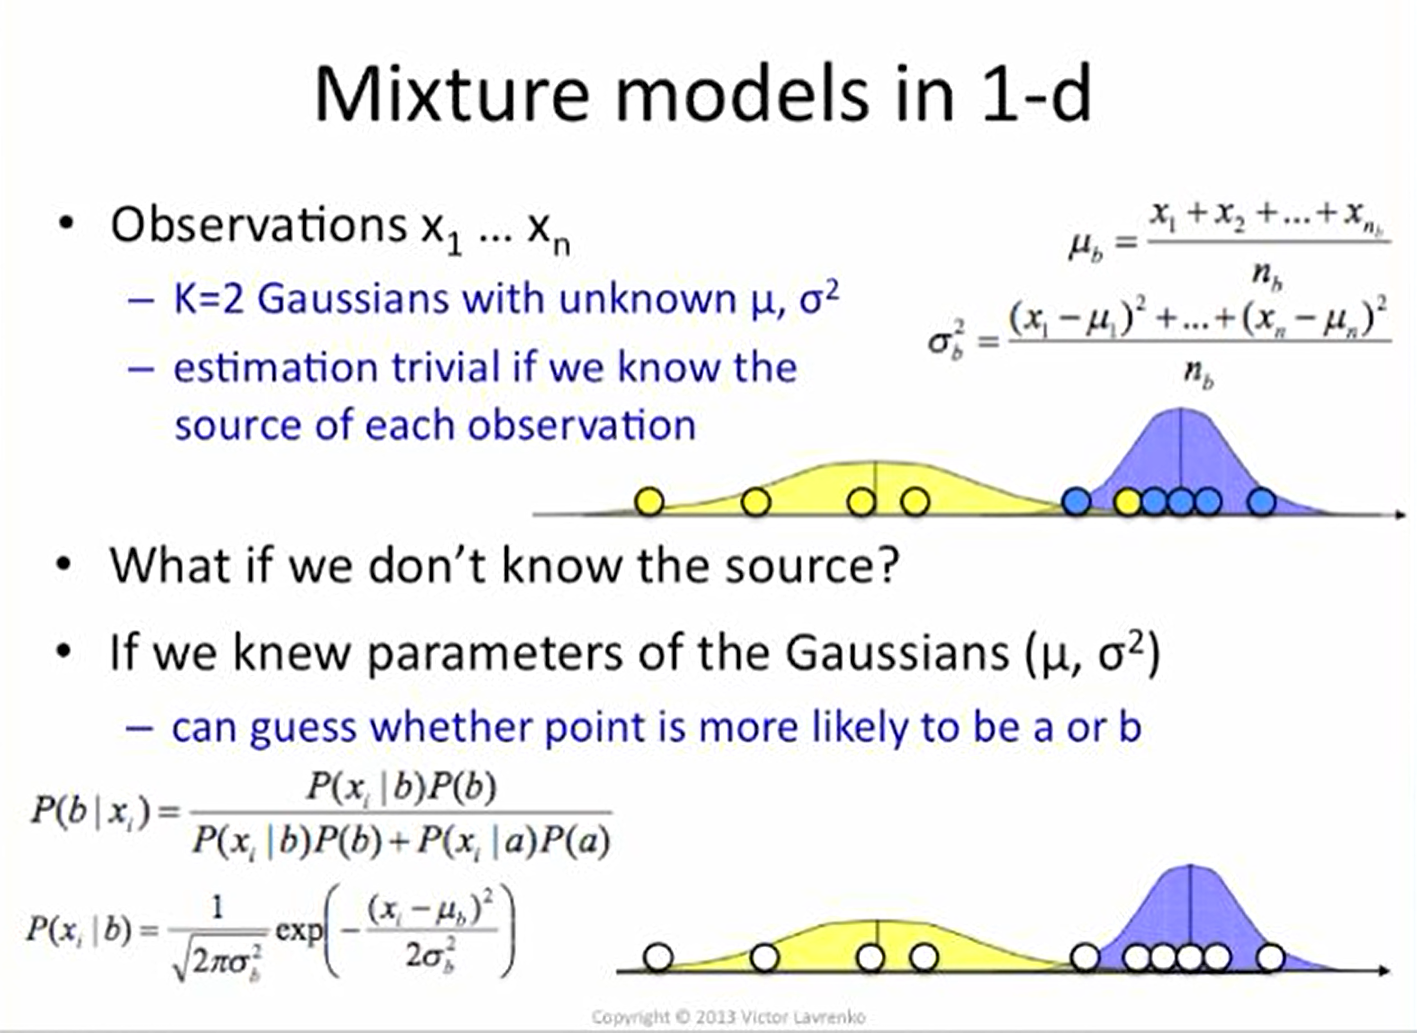
\includegraphics[width=0.5\linewidth]{images/1d_mixture_models}
	\label{fig:1d_mixture_models}
\end{figure}
\begin{figure}[H]
	\centering
	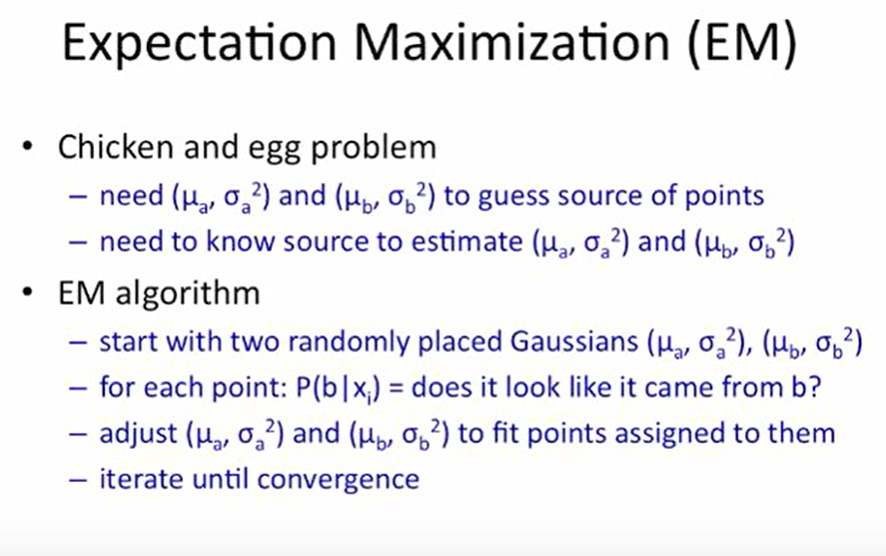
\includegraphics[width=0.5\linewidth]{images/em}
	\label{fig:em}
\end{figure}
\newpage
\subsection{EM Algorithm Process}
\begin{enumerate}
	\item \textbf{Initialization:} Randomly initialize model parameters $p_i,\mu^{(i)},\delta_i^2$
	\item \textbf{Expectation} + Evaluation(Testing): Find new assignments of $p(i|t)$
	\item \textbf{Maximization} + Parameter Estimation (Supervised Learning): Update model parameters $p_i,\mu^{(i)},\sigma_i^2$
\end{enumerate}
We now substitute $\delta(i|t)$ with $p(i|t)$, the probability that $x^{(t)}$ is assigned to $i$.

$$\sum_i^k p(i|t) = 1$$
$$ \sum_{i=1}^k[\sum_{t=1}^n p(i|t)\log(p_i\cdot p(x^{(t)}|\mu^{i}, \sigma^2_i)] $$

\noindent This simple algorithm is guaranteed to monotonically increase the log-likelihood of the data under the mixture model (cf. k-means). Just as in k-means, however, it may only find a locally optimal solution.

\section{Hidden Markov Model (HMM)}

\subsection{Structured Prediction}

$$ f: S_1 \rightarrow S_2$$ 
\begin{align*}
\text{where } & dim(S_1) > dim(S_2)\\
& S_1 \text{ is a structured space consisting of word/observation sequences}\\
& S_2 \text{ is a structured space consisting tag/state sequences}
\end{align*}

\subsection{Computing Joint Likelihood of a HMM}

To calculate the probabilities of the sequence of words ($x_0...x_n$) generated given the tags ($y_0...y_{n+1}$)
$$ p(x_1...x_n, y_0...y_{n+1}) = p(y_0...y_{n+1}) \cdot p(x_1...x_n | y_0 ... y_{n+1}) $$

\noindent We assumed strong independence between the variables such that
$$ p(y_2 | y_1, y_0) \approx p(y_2 | y_1) $$

\noindent Expanding the joint probability terms individually, 
\begin{align*}
	p(y_0 ... y_{n+1}) =& \prod_{j=0}^n p(y_n+1 | y_n)\\
	p(x_1...x_n | y_0 ... y_n+1) =& \prod_{j=1}^n p(x_j|y_j)\\
	\text{Hence, } p(x_1...x_n, y_0...y_{n+1}) =& \prod_{j=0}^n p(y_n+1 | y_n) \cdot \prod_{j=1}^n p(x_j|y_j)
\end{align*}

\noindent For simplicity, we rewrite the notation of individual transmission and emission probabilities.
\begin{align*}
	\text{Transmission Probability } && a_{u,v} &= \frac{\text{count}(u,v)}{\text{count}(u)}\\
	\text{Emission Probability } && b_{u(o)} &= \frac{\text{count}(u\rightarrow o)}{\text{count}(u)}
\end{align*}

\begin{align*}
	\prod_{j=0}^n a_{y_j,y_j+1} &= \prod_{j=0}^n p(y_n+1 | y_n)\\
	\prod_{j=1}^n b_{y_j(x_j)} &= \prod_{j=1}^n p(x_j|y_j)\\
	\text{Joint Probability} &\leftarrow \prod_{j=0}^n a_{y_j,y_j+1} \cdot \prod_{j=1}^n b_{y_j(x_j)}
\end{align*}

\subsection{Supervised Learning}

\subsubsection{Decoding}

Finding most probable label sequence $y$ given the word sequence $x$


\paragraph{Brute Force Enumeration}
\begin{align*}
	y* &= \argmax_y p(y|x)\\
	&= \argmax_y \frac{p(x, y)}{p(x)}\\
	&= \argmax_y p(x,y)
\end{align*}

\noindent This method is not feasible once there are too many label sequences. There will be $O(|T|^n)$ possible sequences.

\paragraph{Viterbi Algorithm}\mbox{}\\
Since the HMM has a simple dependence structure, we can exploit this in a dynamic programming algorithm.

\begin{enumerate}
	\item We initialize $\pi(0,u)$
	\begin{itemize}[label=$\circ$]
		\item $1$ if $u = START$
		\item $0$ otherwise
	\end{itemize}
	\item For $j=0...n-1$, $$ \pi (j+1,u) = \max_v { \pi(j,v) \cdot b_u(x_{j+1}) \cdot a_{v,u} } y_n^* =\argmax_u { \pi(j,u) \cdot a_u,y^*_{j+1}} $$
	\item Finally, $$ \pi (n+1,STOP) = \max_v { \pi(n,v) \cdot a_{v,STOP}) } $$
\end{enumerate}

\noindent\textbf{Time complexity:} $O((n-1)T^2+T=T) = O(nT^2)$

\begin{itemize}
	\item T is the number of nodes in each column, and we carry out n-1 operations for each column.
	\item Calculation for each node is $O(T)$, and do it for $n*t$ nodes so it is $O(T^2)$.
	\item $O(T)$ calculation at start and stop nodes.
\end{itemize}

\noindent\textbf{Space complexity:} $O(nT)$

\subsection{Unsupervised Learning}
We can use EM algorithms to learn model parameters in an unsupervised manner.

\begin{framed}
	\begin{displayquote}
		\begin{center}
			Recall that EM Algorithms seek to maximize likelihood that\\ the data is generated by a mixture model.
		\end{center}
	\end{displayquote}
\end{framed}

\subsubsection{Hard EM}

\paragraph{E-step}

\begin{enumerate}
	\item Assign each observed sequence of outputs (data point) as $x^{(1)}...x^{(m)}$
	\item Assign each $x$ to a single state sequence/tag sequence $y$ (\textit{no partial membership}).
	\item \textit{Decoding:} For each observation sequence, use Viterbi algorithm to find the most probable state sequence $\textbf{y}^{(i)^*}$
\end{enumerate}
$$ Y^* =\argmax_Y P(Y|X) $$

\paragraph{M-step}\mbox{}\\

\noindent Parameter estimation using MLE with labelled data from the E-step 
\begin{align*}
	\text{Transmission Probability } && a_{u,v} &= \frac{count(u,v)}{count(u)} && \text{for any } u,v \in { 0,1,2...N+1}\\
	\text{Emission Probability } && b_{u(o)} &= \frac{count(u\rightarrow o)}{count(u)} && \text{for any } u \in { 0,1,2...N+1}, o \in \sum
\end{align*}

\subsubsection{Soft EM}
For soft EM, we must evaluate a posterior probability over possible tag sequences, so we cannot use Viterbi algorithm.

\begin{itemize}
	\item Viterbi algorithm will result in hard membership (a specific $y$ with max probability) for each observed sequence of outputs.
\end{itemize}

\paragraph{Inference}\mbox{}\\
To compute the posterior possibilities efficiently for any $u\in 1...N, j\in 1...n$,
$$ p(y_j=u|\textbf{x};\theta) = \sum_{\textbf{y}:y_j=u}p(\textbf{y}|\textbf{x};\theta) $$
These probabilities is conditioned on the observed sequence $\textbf{x}$ and the model parameters $\theta$.

\noindent Thereafter,
\begin{align*}
	 \text{Given that } &\sum_B P(A,B) = P(A)\\
	 &\alpha_u(j) = p(x_1...x_{j-1}, y_j=u)\\
	 & \beta_u(j) = p(x_j...x_{n} | y_j=u)
\end{align*}

\begin{align*}
	 p(y_j = u | \textbf{x};\theta) &= \frac{\alpha_u(j)\beta_u(j)}{\sum_v \alpha_v(k)\beta_v(k)}\\
	 p(y_j = u, y_{j+1} = v|\textbf{x};\theta) &= \frac{\alpha_u(j)\cdot b_u{x_j} \cdot a_{u,v} \cdot \beta_v(j+1)}{\sum_v \alpha_v(k)\beta_v(k)}
\end{align*}

\paragraph{Finding the fractional count}

\begin{align*}
	count(u,v) &= \sum_{i=1}^m count^{(i)} (u,v)\\
	&= \sum_{i=1}^m \sum_y p(y|x^{(i)}) count(\textbf{x}^{(i)},y, u \rightarrow v)\\
	&= \sum_{i=1}^m \sum_{j=0}^n p(y_j = u, y_{j+1} = v|\textbf{x}^{(i)})\\
	&= \sum_{i=1}^m \sum_{j=0}^n \frac{\alpha_u(j)\cdot b_u{x_j} \cdot a_{u,v} \cdot \beta_v(j+1)}{\sum_v \alpha_v(k)\beta_v(k)}
\end{align*}

\subsection{Forward-Backward Algorithm}

\subsubsection{Going Forward}
\begin{itemize}
	\item $\alpha_u(j) =$ the sum of the scores of all paths from START to node $u$ at $j$
	\item For the first node, there is no emission probability. 
	\begin{align*}
	\alpha_u(1) &= \alpha_{START,u}\\
	&= p(x_0 , y_1 = u)
	\end{align*}
	\item For the other nodes,
\end{itemize}
$$\text{Given that }\sum_B P(A,B) = P(A)$$
\begin{align*}
\alpha_u(j+1) &= p(x_1 ... x_j, y_{j+1} = u)\\
&= \sum_v p(x_1...x_j, y_{j+1} = u, y_j = v)\\
&= \sum_v p(x_1...x_{j-1}, y_j = v, x_j, y_{j+1}= u)\\
&= \sum_v p(x_1...x_{j-1}, y_j = v) \cdot b_v(x_j) \cdot a_{v,u}\\
&= \sum_v \alpha_v(j) \cdot b_v(x_j)\cdot \alpha_{v,u}
\end{align*}
\newpage
\subsubsection{Going Backward}
\begin{itemize}
	\item $\beta_u(j) =$ the sum of the scores of all paths from node $u$ at $j$ to STOP.
\end{itemize}
\begin{align*}
	\beta_u(j) &= p(x_j...x_n | y_j = u)\\
	&= \sum_v p(x_j...x_n, y_{j+1} = v | y_j = u)\\
	&= \sum_v p(x_j, y_{j+1} = v, x_{j+1}... x_n | y_j =u)\\
	&= \sum_v b_u(x_j) \cdot a_{u,v} \cdot p(x_{j+1}...x_n | y_{j+1} = v)\\
	&= \sum_v b_u(x_j) \cdot a_{u,v} \cdot \beta_v(j+1)
\end{align*}
Time Complexity: $O(nT^2)$
\begin{itemize}
	\item $O(T)$ operations for $T$ nodes at $n$ positions
\end{itemize}
Time complexity of 1 EM iteration: $O(mnT^2)$\\
\\
\noindent Forward Backward Algorithm is a type of Inside-Outside Algorithm, which the Prof will only cover in NLP course.

\section{Forward-Backward Algorithm}
\subsection{Going Forward}
\begin{itemize}
	\item $\alpha_u(j) =$ the sum of the scores of all paths from START to node $u$ at $j$
	\item For the first node, there is no emission probability. 
	\begin{align*}
		\alpha_u(1) &= \alpha_{START,u}\\
		&= p(x_0 , y_1 = u)
	\end{align*}
	\item For the other nodes,
\end{itemize}
$$\text{Given that }\sum_B P(A,B) = P(A)$$
\begin{align*}
	\alpha_u(j+1) &= p(x_1 ... x_j, y_{j+1} = u)\\
	&= \sum_v p(x_1...x_j, y_{j+1} = u, y_j = v)\\
	&= \sum_v p(x_1...x_{j-1}, y_j = v, x_j, y_{j+1}= u)\\
	&= \sum_v p(x_1...x_{j-1}, y_j = v) \cdot b_v(x_j) \cdot a_{v,u}\\
	&= \sum_v \alpha_v(j) \cdot b_v(x_j)\cdot \alpha_{v,u}
\end{align*}
\newpage
\subsection{Going Backward}
\begin{itemize}
	\item $\beta_u(j) =$ the sum of the scores of all paths from node $u$ at $j$ to STOP.
\end{itemize}
\begin{framed}
	\begin{displayquote}
		\begin{center}
			$x_{j+1}$ cannot be generated before $x_j$
		\end{center}
	\end{displayquote}
\end{framed}
\begin{align*}
	\beta_u(j) &= p(x_j...x_n | y_j = u)\\
	&= \sum_v p(x_j...x_n, y_{j+1} = v | y_j = u)\\
	&= \sum_v p(x_j, y_{j+1} = v, x_{j+1}... x_n | y_j =u)\\
	&= \sum_v b_u(x_j) \cdot a_{u,v} \cdot p(x_{j+1}...x_n | y_{j+1} = v)\\
	&= \sum_v b_u(x_j) \cdot a_{u,v} \cdot \beta_v(j+1)
\end{align*}
Time Complexity: $O(nT^2)$
\begin{itemize}
	\item $O(T)$ operations for $T$ nodes at $n$ positions
\end{itemize}

\section{Bayesian Networks}
Bayesian networks are generative probabilities models that are developed for representing and using probabilistic information. Bayesian networks subsume mixture models, HMMs and many others.

\begin{enumerate}
	\item Bayesian Networks are \textbf{Directed Acyclic Graphs} (DAG) over the variables.
	\begin{itemize}[label=$\circ$]
		\item We usually generate the graph from $x_1$ first, and each node $x_i$ has a Conditional Probability Distribution $P(X_i | \arg P(X_i))$.
		\item If there is a directed edge from $x_1 \rightarrow$ $x_3$, then $x_1$ is a parent of $x_3$. And once we know the parents, we can write the probability distribution over all the variables with chain rule as
		$$ P(X_1=x_1,...,X_d = x_d) = \prod_{i=1}^d P(X_i = x_i|\arg P(X_i))$$
	\end{itemize}
\end{enumerate}
\begin{framed}
	\begin{displayquote}
		\begin{center}
			Cannot have cyclic graphs, as it will result in weird probabilities like $p(x_3|x_3)$. This is simply not valid!! Generative Models typically have DAGs.
		\end{center}
	\end{displayquote}
\end{framed}
\begin{enumerate}[label=\arabic*.,start=2]
	\item The network will have the \textbf{associated probability distribution}.
	\begin{enumerate}[label=\roman*.]
		\item For each node $i$, we will attach a table of probabilities containing the combination of assignment of values that has been calculated up to node $i$.
		\item As $i$ increases, the table of probabilities attached to node $i$ expands.
		\item Each row in the table must add up to $1$.
		\item This is similar to $b_u(o)$.
	\end{enumerate}
\end{enumerate}

\subsection{Independence in Bayesian Networks}
If there is a direct edge from A to B, influence can flow from X to Y regardless of whether other variables are observed. They would never be independent.\\
\\
\noindent \textit{Basic Independence Rule}\\
\\
\noindent If A and B are conditionally independent, $ P(A,B) = P(A)\cdot P(B) $ $P(A|B) = P(A) $\\
\\
\noindent To prove dependence, just show a case where $P(A|B) \not = P(A)$.

\subsubsection{Summary: X and Z dependence}
For the examples below,
\begin{itemize}
	\item \img{images/26AA} refers to known variable,
	\item \img{images/26AB} refers to unknown variable,
	\item $\rightarrow$: causal direction
	\item $\leftarrow$: evidential direction
\end{itemize}

\begin{table}[H]
	\centering
	\begin{tabular}{|c|c|c|}
		\hline
		\textbf{Relationship}         & \textbf{Y is not given}                                                                                                                                              & \textbf{Y is given}                                                                                                                                                  \\ \hline
		X$\rightarrow$Y$\rightarrow$Z & \cincludegraphics[height=0.5cm]{images/2714}: \cincludegraphics[height=0.5cm]{images/26AA}$\rightarrow$\cincludegraphics[height=0.5cm]{images/26AA}$\rightarrow$\cincludegraphics[height=0.5cm]{images/26AA} & \cincludegraphics[height=0.5cm]{images/2715}: \cincludegraphics[height=0.5cm]{images/26AA}$\rightarrow$\cincludegraphics[height=0.5cm]{images/26AB}$\rightarrow$\cincludegraphics[height=0.5cm]{images/26AA} \\ \hline
		X$\leftarrow$Y$\rightarrow$Z  & \cincludegraphics[height=0.5cm]{images/2714}: \cincludegraphics[height=0.5cm]{images/26AA}$\leftarrow$\cincludegraphics[height=0.5cm]{images/26AA}$\rightarrow$\cincludegraphics[height=0.5cm]{images/26AA} & \cincludegraphics[height=0.5cm]{images/2715}: \cincludegraphics[height=0.5cm]{images/26AA}$\leftarrow$\cincludegraphics[height=0.5cm]{images/26AB}$\rightarrow$\cincludegraphics[height=0.5cm]{images/26AA} \\ \hline
		X$\rightarrow$Y$\leftarrow$Z  & \cincludegraphics[height=0.5cm]{images/2715}: \cincludegraphics[height=0.5cm]{images/26AA}$\rightarrow$\cincludegraphics[height=0.5cm]{images/26AA}$\leftarrow$\cincludegraphics[height=0.5cm]{images/26AA}    & \cincludegraphics[height=0.5cm]{images/2714}: \cincludegraphics[height=0.5cm]{images/26AA}$\rightarrow$\cincludegraphics[height=0.5cm]{images/26AB}$\leftarrow$\cincludegraphics[height=0.5cm]{images/26AA} \\ \hline
	\end{tabular}
\end{table}
\begin{framed}
	\begin{displayquote}
		\begin{center}
			Just remember one column and you can derive the other column.
		\end{center}
	\end{displayquote}
\end{framed}

\subsubsection{Chain: X$\rightarrow$Y$\rightarrow$Z}
\img{images/26AA}$\rightarrow$\img{images/26AB}$\rightarrow$\img{images/26AA}: to prove $X, Z$ are independent. (This is hard to prove) $$ P(X,Z) = P(X) \cdot P(Z) $$
\img{images/26AA}$\rightarrow$\img{images/26AA}$\rightarrow$\img{images/26AA}: to prove $X, Z$ are independent.
$$P(X,Z|Y) = P(X|Y) \cdot P(Z|Y)$$
\newpage
\noindent To prove that the conditional dependence of Z and Y is not affected regardless of Y having a parent, $$ P(Z|Y,X) = P(Z|Y) $$
\noindent We can calculate as follows:
\begin{align*}
	P(X,Y,Z) &= P(X)\cdot P(Y|X) \cdot P(Z|Y)\\
	P(Z|Y,X) &= \frac{P(X,Y,Z)}{P(X,Y)}\\
	&= \frac{P(X)\cdot P(Y|X) \cdot P(Z|Y)}{P(X,Y)}\\
	&= \frac{P(X)\cdot P(Y|X) \cdot P(Z|Y)}{P(X) \cdot P(Y|X)}\\
	&= P(Z|Y)
\end{align*}
\begin{itemize}
	\item Hence, Y is known as an open gate.
\end{itemize}

\subsubsection{Common Parent (Common Cause)}
$Y$ has a directed edge to both $X,Z$.
\begin{itemize}
	\item \img{images/26AA}$\leftarrow$\img{images/26AB}$\rightarrow$\img{images/26AA}: we cannot prove that $X,Z$ are independent.
	\item \img{images/26AA}$\leftarrow$\img{images/26AA}$\rightarrow$\img{images/26AA}: $X,Z$ are independent.
	\item Here, Y is an \textbf{open gate}.
\end{itemize}

\subsubsection{Common Child (Explaining Away)}
\begin{framed}
	\begin{displayquote}
		Explaining away is a common pattern of reasoning in which the confirmation of one cause of an observed or believed event \textbf{reduces the need to invoke alternative causes}. The opposite of explaining away also can occur, where the confirmation of one cause increases belief in another.
	\end{displayquote}
\end{framed}
Both $X,Z$ have a directed edge to $Y$.
\begin{itemize}
	\item \img{images/26AA}$\rightarrow$\img{images/26AB}$\leftarrow$\img{images/26AA}: $X,Z$ are independent.
	\item \img{images/26AA}$\rightarrow$\img{images/26AA}$\leftarrow$\img{images/26AA}: $X,Z$ are not independent.
	\item Hence, Y is a \textbf{open gate}.
\end{itemize}
\newpage
\subsubsection{Examples}
\paragraph{Earthquake + Burglary}\mbox{}\\
\begin{figure}[H]
	\centering
	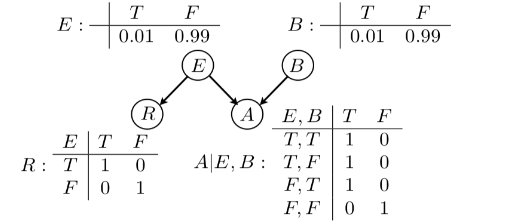
\includegraphics[width=0.7\linewidth]{images/bayesian_network_example}
	\label{fig:bay_network}
\end{figure}
\noindent Here, $E$ and $B$ have a common child $A$, and $E$ is the common parent of $R$ and $A$.
\begin{align*}
	P(B=T|A=T) &= \frac{P(B=T,A=T)}{\sum_{b\in{T,F}}P(B=b,A=T)}\\
	&= 0.5025\\
	P(B=b, A=T, E=T) &= P(E=T) \cdot P(A=T | E=T, B=T)\\
	&= 0.99 \cdot 0.01 \cdot 1\\
	P(B=b |A=T, E=T) &= \frac{P(B=b, A=T,E=T)}{P(A=T,E=T)}\\
	&= \frac{0.01 \cdot 0.01}{0.99\cdot 0.01 + 0.01\cdot 0.01}\\
	&= 0.01
\end{align*}
\paragraph{President and Traffic Accident}\mbox{}\\
\begin{figure}[H]
	\centering
	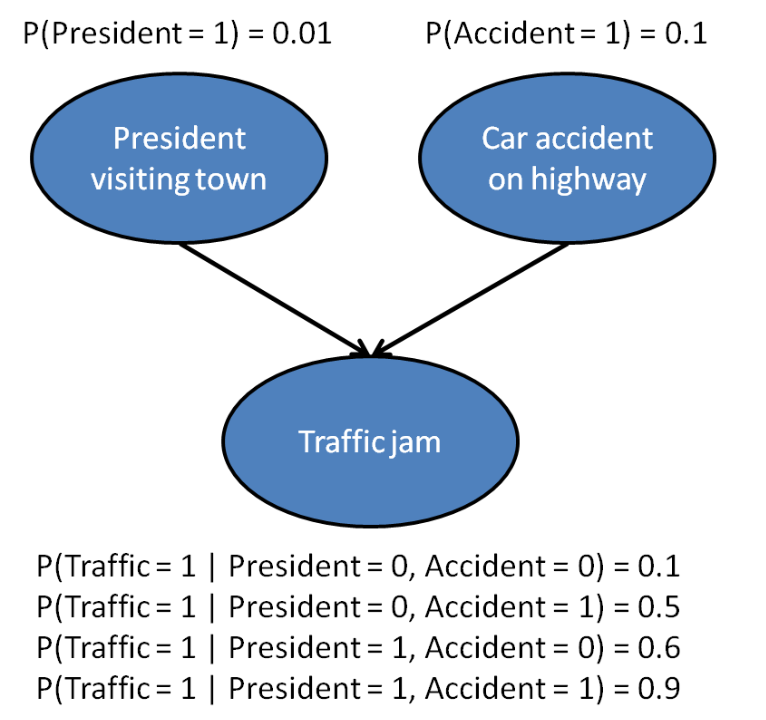
\includegraphics[width=0.5\linewidth]{images/pres_accident}
	\label{fig:pres_accident}
\end{figure}
\begin{table}[H]
	\centering
	\begin{tabular}{|c|c|c|c|c|}
		\hline
		& \textbf{\begin{tabular}[c]{@{}c@{}}President = 0, \\ Accident = 0\end{tabular}} & \textbf{\begin{tabular}[c]{@{}c@{}}President = 1, \\ Accident = 0\end{tabular}} & \textbf{\begin{tabular}[c]{@{}c@{}}President = 0, \\ Accident = 1\end{tabular}} & \textbf{\begin{tabular}[c]{@{}c@{}}President = 1, \\ Accident = 1\end{tabular}} \\ \hline
		Traffic = 1 & 0.1                                                                             & 0.6                                                                             & 0.5                                                                             & 0.9                                                                             \\ \hline
		Traffic = 0 & 0.9                                                                             & 0.4                                                                             & 0.5                                                                             & 0.1                                                                             \\ \hline
	\end{tabular}
\end{table}

\subsection{Bayes Ball Algorithm}
As long we can find a path to connect $X$ and $Y$ that are open gates, we can conclude $X$ and $Y$ are dependent.

\subsubsection{Markov Net}
A Markov Net comprises of a particular node $x_i$'s parents, co-parents and children. Node $x_i$ is independent of all other nodes outside this Markov net.

\subsection{Bayesian Information Criterion (BIC)}
BIC is a model selection criterion for comparing 2 different Bayesian networks, where
\begin{itemize}
	\item $dim(G) =$ the number of independent parameters in the model
	\item $m =$ the number of data points in the training set
	\item $r_j \forall j\in pa_i =$ the size of the probability table $\theta_i(x_i|\textbf{x}_{pa_i})\ -\ \text{the number of associated normalization constraints}$ $$ BIC(D;\theta,G) = l(D;\theta,G) - \frac{dim(G)}{2} \log(m) $$
\end{itemize}
\noindent We then search for the graph $G$ that \textbf{maximizes} $BIC(D;\theta,G)$.
\begin{enumerate}
	\item With the complete data, find conditional estimates for each variable and the parent selection scores for each variable. $$\theta_i(x_i|x_{pa_i}) , score(i|pa_i;D)$$
	\item Find the decomposable scoring function for graphs. $$ score(G;D) = \sum_{i=1}^d score(i|pa_i,D) $$
	\item Find highest scoring \textbf{acyclic graph}.
\end{enumerate}
$$\argmax_G score(G;D) $$
\newpage
\section{Reinforcement Learning}
\noindent \textbf{Problem:} $f: S \rightarrow A$
\begin{itemize}
	\item $S$: Set of States
	\item $A$: Set of Actions
\end{itemize}
\noindent \textbf{Transition Probability}
\begin{itemize}
	\item Moving from one state to another state is not definite
	\item $T(s,a,s') = p(s'|s,a)$
\end{itemize}
\noindent \textbf{Reward}
\begin{itemize}
	\item Incentivize a target state to be reached / not reached.
	\item Can be positive (reward) / negative (penalty)
	\item $R(s,a,s')$: Generally
	\item $R(s')$ : if the system only requires the target state to be reached.
\end{itemize}

\subsection{Markov Decision Process}
Given
\begin{itemize}
	\item a set of states $S$
	\item a set of actions $A$
	\item a transition probability function $T(s,a,s') = p(s'|s,a) $
	\item a reward function $R(s,a,s')$ or $R(s')$
\end{itemize}

\subsubsection{Utility (Long Term Reward)}
\begin{itemize}
	\item Maximizing the rewards alone is not sufficient to incentivise the program to reach the final state that you want. The program may infinitely loop around a few states.
	\item Hence we apply a \textbf{discount} $\gamma$ to long-term rewards.
\end{itemize}
\begin{align*}
	U([s_1,s_2,...s_n]) &= R(s_1) + \gamma R(s_2) + \gamma_2 R(s_3) + \ldots\\
	&= \sum_{t=0}^\infty R(s_t)
\end{align*}
\newpage
\subsubsection{Value Iteration Policy}
We first define the following:
\begin{itemize}
	\item $\pi(s)$: a particular policy that specifies the action we should take in state $s$
	\item $V^\pi(s)$: The value of state $s$ under policy $\pi$
	\item $Q^\pi(s,a)$: The $Q$-value of state $s$ and action $a$ under policy $\pi$
\end{itemize}
and the optimal version of them:
\begin{itemize}
	\item $\pi^*(s)$: a particular policy that specifies the action we should take in state $s$
	\item $V^*(s)$: The value of state $s$ under the optimal policy $\pi^*$
	\item $Q^*(s,a)$: The $Q$-value of state $s$ and action $a$ under policy $\pi^*$
\end{itemize}
\begin{align*}
	Q^*(s,a) &= \sum_{s'} T(s,a,s') [R(s,a,s') + \gamma V^*(s')]\\
	V^*(s) &= Q^*(s,\pi^*(s))\\
	&= \max_a Q^*(s,a)\\
	&= \max_a \sum_{s'} T(s,a,s') [R(s,a,s') + \gamma V^*(s')]\\
	\pi^*(s) &= \argmax_a Q^*(s,a)
\end{align*}

\subsubsection{Value Iteration Algorithm}
\begin{enumerate}
	\item Start with $V_0^*(s) = 0$ $\forall s \in S$
	\item Given $V_i^*$,
	\begin{enumerate}[label=\roman*.]
		\item calculate the values for all states $s \in S$ and
		\item keep track of the best actions to formulate the best policy
	\end{enumerate}
	$$ 
	V^*(s) \leftarrow \max_a \sum_{s'} T(s,a,s') [R(s,a,s') + \gamma V^*(s')] 
	$$
	\item Repeat until convergence.
\end{enumerate}

\subsubsection{Q-value Iteration Algorithm}
Similar to Value Iteration Algorithm.
\end{document}